\documentclass[tikz,border=8pt]{standalone}
\usepackage{amsmath,amssymb}
\usetikzlibrary{arrows.meta,automata,positioning,quotes}
\begin{document}
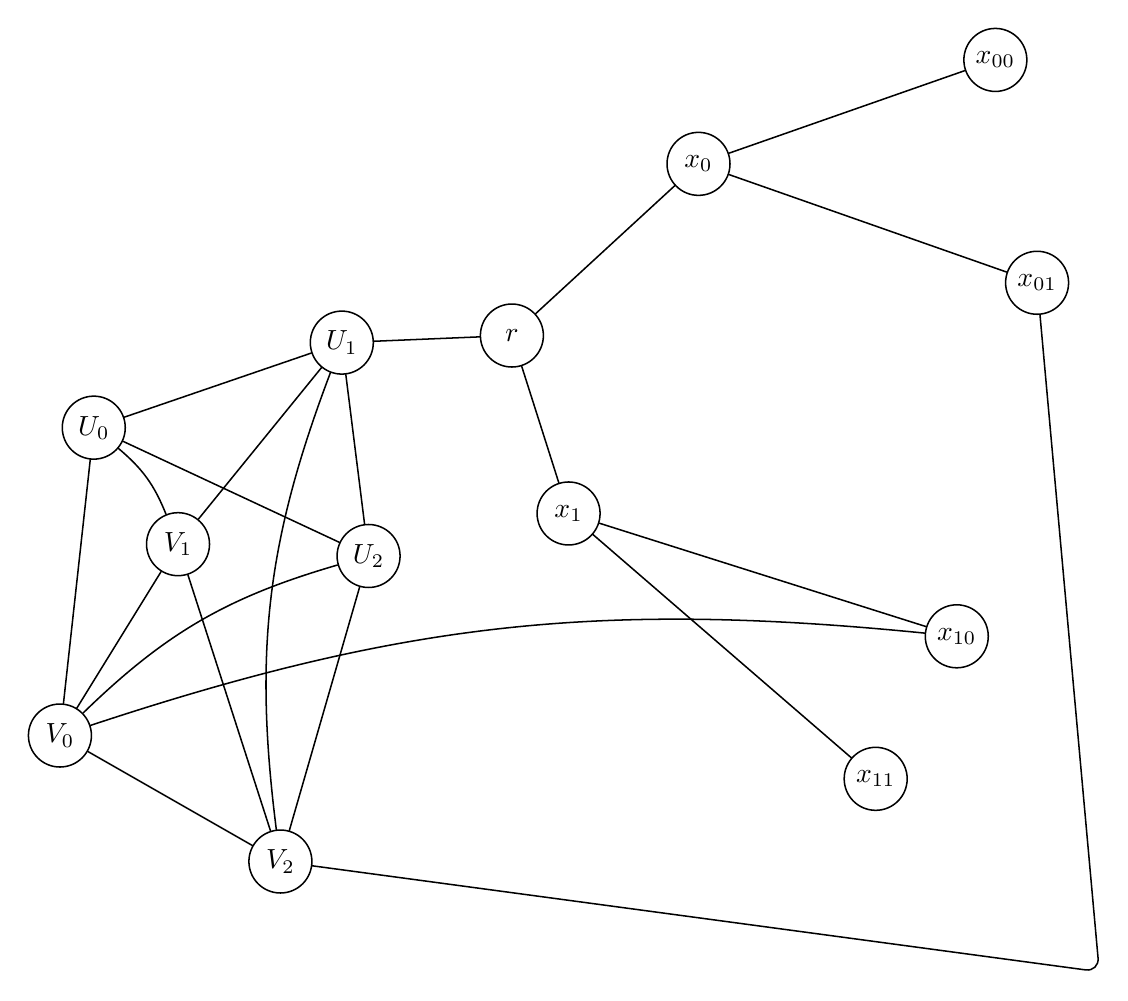
\begin{tikzpicture}[x=1cm,y=1cm]
\tikzset{
  graphnode/.style={circle,draw=black,line width=0.55pt,minimum size=8mm,inner sep=1pt,font=\sffamily},
  graphedge/.style={draw=black,line width=0.55pt,line cap=round,line join=round},
  directed/.style={graphedge,-{Stealth[length=2.4mm,width=2.0mm]}},
  undirected/.style={graphedge}
}
\node[graphnode] (n_U0) at (-7.57,1.91) {$U_0$};
\node[graphnode] (n_U1) at (-4.42,2.99) {$U_1$};
\node[graphnode] (n_U2) at (-4.08,0.28) {$U_2$};
\node[graphnode] (n_V0) at (-8.00,-2.00) {$V_0$};
\node[graphnode] (n_V1) at (-6.50,0.43) {$V_1$};
\node[graphnode] (n_V2) at (-5.20,-3.60) {$V_2$};
\node[graphnode] (n_r) at (-2.26,3.08) {$r$};
\node[graphnode] (n_x0) at (0.11,5.26) {$x_0$};
\node[graphnode] (n_x1) at (-1.54,0.82) {$x_1$};
\node[graphnode] (n_x00) at (3.88,6.58) {$x_{00}$};
\node[graphnode] (n_x01) at (4.41,3.75) {$x_{01}$};
\node[graphnode] (n_x10) at (3.39,-0.74) {$x_{10}$};
\node[graphnode] (n_x11) at (2.36,-2.55) {$x_{11}$};
\draw[undirected] (n_U0) -- (n_U1);
\draw[undirected] (n_U1) -- (n_U2);
\draw[undirected] (n_U0) -- (n_U2);
\draw[undirected] (n_V0) -- (n_V1);
\draw[undirected] (n_V1) -- (n_V2);
\draw[undirected] (n_V0) -- (n_V2);
\draw[undirected] (n_U0) -- (n_V0);
\draw[undirected] (n_U1) -- (n_V1);
\draw[undirected] (n_U2) -- (n_V2);
\draw[undirected] (n_U0) to[bend left=14] (n_V1);
\draw[undirected] (n_U1) to[bend right=14] (n_V2);
\draw[undirected] (n_U2) to[bend right=14] (n_V0);
\draw[undirected] (n_U1) -- (n_r);
\draw[undirected] (n_r) -- (n_x0);
\draw[undirected] (n_r) -- (n_x1);
\draw[undirected] (n_x0) -- (n_x00);
\draw[undirected] (n_x0) -- (n_x01);
\draw[undirected] (n_x1) -- (n_x10);
\draw[undirected] (n_x1) -- (n_x11);
\draw[undirected,rounded corners=5pt] (n_V2) -- (5.20,-5.00) -- (n_x01);
\draw[undirected] (n_V0) to[bend left=12] (n_x10);
\end{tikzpicture}
\end{document}
